\documentclass[a4paper,12pt]{article}
\usepackage{fancyhdr}
\usepackage{lastpage}
\usepackage{geometry}
\usepackage{listings}
\usepackage{datetime}
\usepackage{xeCJK}
\usepackage{hyperref}
\usepackage{amsmath}
\usepackage{graphicx}
\usepackage{float} % 加入 float 宏包以使用 [H]
\usepackage{longtable}

\geometry{left=2.5cm, right=2.5cm, top=2.5cm, bottom=2.5cm}
\pagestyle{fancy}
\setCJKmainfont{Noto Sans CJK HK}
% 英文字體 consolas
\setmonofont{Consolas}
% 設定內文文字大小
\renewcommand{\normalsize}{\fontsize{12pt}{\baselineskip}\selectfont}

% 設定頁首
\fancyhf{}
\fancyhead[L]{牛頓法 2D 視覺化}
\fancyhead[R]{\today}
\fancyfoot[C]{\thepage/\pageref{LastPage}}

\title{牛頓法 2D 視覺化程式文件}
\author{01057033洪銘均}
\date{\today}

\begin{document}
\maketitle
\tableofcontents
\newpage

\section{程式概述}
本程式使用 OpenGL 和 GLSL 來視覺化牛頓法在二維空間中的迭代過程,將函數圖形與迭代點顯示在螢幕上,以便於觀察牛頓法的收斂情況。程式包含若干主要組件,包括 GLSL 著色器、算法實現、以及視覺化部分。

\section{檔案與功能}
以下是每個原始碼檔案的簡要描述:

\subsection{GLSL 著色器檔案}
\begin{itemize}
    \item \textbf{func\_frag.glsl}:渲染函數圖形的片段著色器,用於控制圖形顏色等視覺效果。
    \item \textbf{func\_vert.glsl}:渲染函數圖形的頂點著色器,負責將頂點座標傳遞給片段著色器。
    \item \textbf{point\_frag.glsl}:渲染牛頓法迭代點的片段著色器,控制點的顏色和透明度。
    \item \textbf{point\_vert.glsl}:渲染牛頓法迭代點的頂點著色器,將點的位置資料傳給片段著色器。
\end{itemize}

\subsection{C++ 標頭檔案}
\begin{itemize}
    \item \textbf{GLinclude.h}:包含 OpenGL 與相關庫的初始化和設定程式碼。
    \item \textbf{glsl.h}:包含編譯和管理 GLSL 著色器的函式。
    \item \textbf{newton2d.h}:定義類別和函式,用於實現牛頓法的計算邏輯,新增以下類別:
    % 在newton2d.h item底下加入以下內容
    \begin{itemize}
        \item \texttt{struct term}: 用於表示函數的係數和次方。
        \item \texttt{Vector2d}: 用於表示二維向量的類別。
        \item \texttt{Polynomial}: 用於表示多項式函數的類別。
        \item \texttt{PolynomialMatrix2d}: 用於表示二維多項式函數的類別。
        \item \texttt{Matrix2d}: 用於表示二維矩陣的類別。
    \end{itemize}
    \item \textbf{visualize.h}:定義類別和函式,用於實現 OpenGL 視覺化功能,新增以下類別:
    % 在visualize.h item底下加入以下內容
    \begin{itemize}
        \item \texttt{struct Vertex}: 用於表示 OpenGL 頂點的結構。
    \end{itemize}
\end{itemize}

\subsection{C++ 實作檔案}
\begin{itemize}
    \item \textbf{glsl.cpp}:實現 GLSL 著色器的載入和編譯邏輯。
    \item \textbf{main.cpp}:程式的主入口,負責初始化 OpenGL 環境並呼叫其他模組完成繪製。
    \item \textbf{newton2d.cpp}:實作牛頓法的具體計算步驟,更新每次迭代的點位置。
    \item \textbf{visualize.cpp}:負責實現圖形視覺化功能,包括調用 OpenGL 繪製 API。
\end{itemize}

\section{函式功能描述}
以下是主要函式的功能說明:

\subsection{glsl.cpp}
\begin{itemize}
    \item \texttt{read\_source\_codes(char *filename)}: 讀取 GLSL 程式碼,return char *。
    \item \texttt{print\_shader\_info\_log(GLenum obj)}: 編譯 GLSL 程式碼。
    \item \texttt{print\_prog\_info\_log(GLenum obj)}: 編譯 GLSL 程式碼。
    \item \texttt{setGLSLshaders(char *vertexShaderFileName, char *fragmentShaderFileName)}: 設置 GLSL 程式碼,return GLuint。
\end{itemize}
\subsection{main.cpp}
\begin{itemize}
    \item \texttt{main()}: 初始化 OpenGL 環境,載入著色器,並進行主迴圈以顯示牛頓法視覺化。
\end{itemize}

\subsection{newton2d.cpp}
\begin{itemize}
    \item \texttt{overload <<}: 重載運算子,用於輸出多項式函數的內容。
    \item \texttt{get\_partial\_derivative(Polynomial, char)}: 計算多項式函數的偏導數,return Polynomial。
    \item \texttt{get\_jacobian\_matrix(Polynomial, Polynomial)}: 計算雅可比矩陣,return PolynomialMatrix2d。
    \item \texttt{get\_func\_value(Polynomial, Vector2d)}: 計算多項式函數在給定點的值,return double。
    \item \texttt{get\_jacobian\_value(PolynomialMatrix2d, Vector2d)}: 計算雅可比矩陣在給定點的值,return Matrix2d。
    \item \texttt{newton2d(Polynomialm Polynomial, Vector2d)}: 實現牛頓法的迭代過程,return std::vector<Vector2d>。
\end{itemize}

\subsection{visualize.cpp}
\begin{itemize}
    \item \texttt{set\_point\_vbo()}: 設置迭代點的 VBO。
    \item \texttt{update\_point\_vbo()}: 更新迭代點的 VBO。
\end{itemize}

\section{UI 說明}
% 插入圖片
\begin{figure}[h]
    \centering
    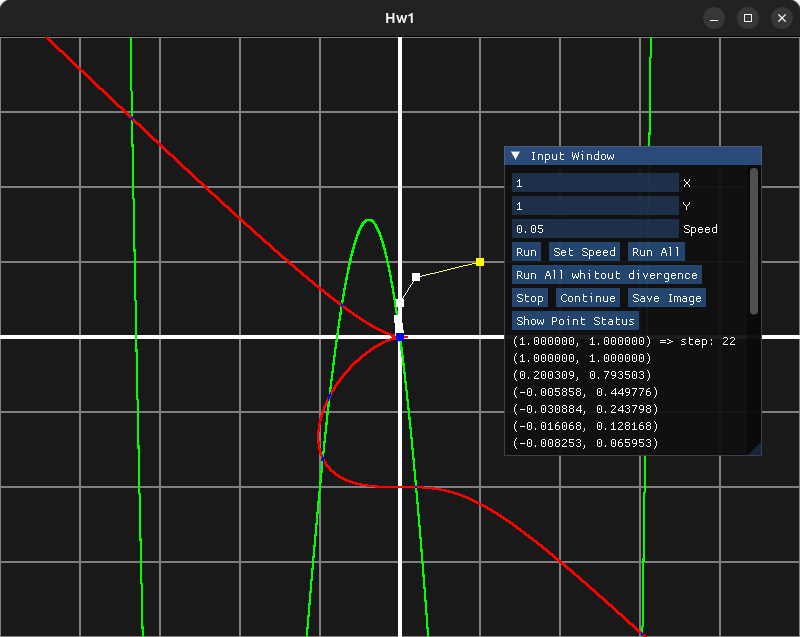
\includegraphics[width=0.8\textwidth]{img/image.png}
    \caption{程式運行截圖,該截圖f(x) = x^3 / 9 + y^3 / 10 + y^2 / 5, g(x) = x^4 + x^3 - 10x^2 - 8x - y }
\end{figure}
%f(x, y) = (x * x * x) / 9.0 + (y * y * y) / 10.0 + (y * y) / 5.0;
%g(x, y) = x * x * x * x + x * x * x - x * x * 10 - 8 * x - y;

\begin{itemize}
    \item \textbf{Run}: 用於開始牛頓法的迭代過程,起始點為輸入框X和Y的值。
    \item \textbf{Set Speed}: 用於設置牛頓法動畫的迭代速度。
    \item \textbf{Run All}: 用於開始牛頓法的迭代過程,並逐一顯示每個迭代點。
    \item \textbf{Run All without divergence}: 用於開始牛頓法的迭代過程,並逐一顯示每個迭代點,在X為0時加入1e-6的偏移。
    \item \textbf{Stop}: 用於停止牛頓法動畫的迭代過程。
    \item \textbf{Continue}: 用於繼續牛頓法動畫的迭代過程。
    \item \textbf{Save Image}: 用於保存當前視窗的畫面。
    \item \textbf{Show Point Status}: 用於所有起使點的迭代結果。
\end{itemize}

\section{心得}
這次得作業實做牛頓2D的計算過程,牛頓法在上課時聽得沒很懂,也是到時做前才搞懂流程。在實做中利用到矩陣運算庫Eigen來完成部份矩陣操作包含反矩陣、矩陣乘法等。在視覺化上,我利用GLSL差值來完成函數和收斂點過程圖形的繪製,雖然一開始遇到線條粗細不一,特定情況下還會出現函數扭曲,但後來加上fwidth就成功修正這問題了。
在後續也嘗試不同的函數來觀察收斂過程,雖然在過程中出現與預期收斂結果不同的情況,在偵錯過程中發現偏微分計算結果有問題,持續追查才發現是我函數初始格式錯誤,後續解決後也正常執行了。

\section{運行結果}
% 插入第二張圖片並強制位置
\begin{figure}[H]
    \centering
    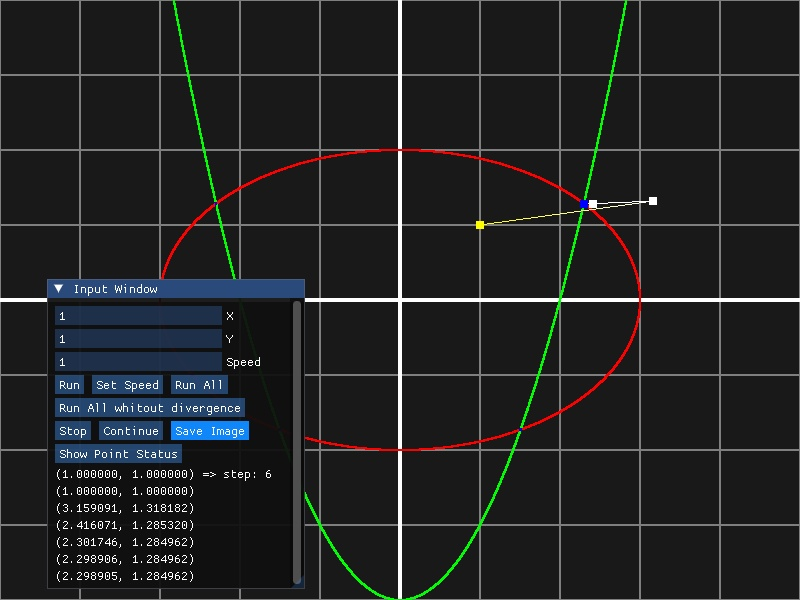
\includegraphics[width=0.8\textwidth]{img/image2.jpg}
    \caption{程式運行截圖,該截圖f(x) = x^2 / 9 + y^2 / 4 - 1, g(x) = x^2 - y - 4 }
\end{figure}

\subsection{P1-1}
% 使用 [H] 強制表格位置
\begin{table}[H]
    \centering
    \begin{tabular}{|c|c|c|}
        \hline
        Point & X & Y \\
        \hline
        P1 & 2.0 & 1.0 \\
        \hline
        P2 & 2.32954545 & 1.31818182 \\
        \hline
        P3 & 2.29918296 & 1.28532042 \\
        \hline
        P4 & 2.29890460 & 1.28496226 \\
        \hline
    \end{tabular}
\end{table}

\subsection{P1-2、P1-3}
% 使用 [H] 強制表格位置
\begin{longtable}{|c|c|c|c|c|c|}
    \hline
    Start Point & X & Y &  End Point X & End Point Y & times\\
    \hline
    P1 & -4 & -3 & -1.50684881 & -1.72940666 & 6 \\ 
    \hline
    P2 & -4 & -2 & -1.50684881 & -1.72940666 & 6 \\ 
    \hline
    P3 & -4 & -1 & -1.50684881 & -1.72940666 & 6 \\ 
    \hline
    P4 & -4 & 0 & -2.29890457 & 1.28496224 & 7 \\ 
    \hline
    P5 & -4 & 1 & -2.29890457 & 1.28496222 & 5 \\ 
    \hline
    P6 & -4 & 2 & -2.29890457 & 1.28496222 & 5 \\ 
    \hline
    P7 & -4 & 3 & -2.29890470 & 1.28496249 & 5 \\ 
    \hline
    P8 & -3 & -3 & -1.50684881 & -1.72940667 & 5 \\ 
    \hline
    P9 & -3 & -2 & -1.50684887 & -1.72940666 & 5 \\ 
    \hline
    P10 & -3 & -1 & -1.50684880 & -1.72940670 & 5 \\ 
    \hline
    P11 & -3 & 0 & -2.29890457 & 1.28496224 & 7 \\ 
    \hline
    P12 & -3 & 1 & -2.29890519 & 1.28496226 & 4 \\ 
    \hline
    P13 & -3 & 2 & -2.29890457 & 1.28496222 & 5 \\ 
    \hline
    P14 & -3 & 3 & -2.29890464 & 1.28496249 & 5 \\ 
    \hline
    P15 & -2 & -3 & -1.50684881 & -1.72940667 & 5 \\ 
    \hline
    P16 & -2 & -2 & -1.50684911 & -1.72940667 & 4 \\ 
    \hline
    P17 & -2 & -1 & -1.50684880 & -1.72940670 & 5 \\ 
    \hline
    P18 & -2 & 0 & -2.29890457 & 1.28496224 & 7 \\ 
    \hline
    P19 & -2 & 1 & -2.29890460 & 1.28496226 & 4 \\ 
    \hline
    P20 & -2 & 2 & -2.29890457 & 1.28496222 & 5 \\ 
    \hline
    P21 & -2 & 3 & -2.29890464 & 1.28496249 & 5 \\ 
    \hline
    P22 & -1 & -3 & -1.50684881 & -1.72940667 & 5 \\ 
    \hline
    P23 & -1 & -2 & -1.50684881 & -1.72940666 & 5 \\ 
    \hline
    P24 & -1 & -1 & -1.50684880 & -1.72940670 & 5 \\ 
    \hline
    P25 & -1 & 0 & -2.29890457 & 1.28496224 & 7 \\ 
    \hline
    P26 & -1 & 1 & -2.29890457 & 1.28496222 & 6 \\ 
    \hline
    P27 & -1 & 2 & -2.29890457 & 1.28496222 & 6 \\ 
    \hline
    P28 & -1 & 3 & -2.29890457 & 1.28496222 & 6 \\ 
    \hline
    P29 & 0 & -3 & inf & -nan & 2 \\ 
    \hline
    P30 & 0 & -2 & -nan & -nan & 2 \\ 
    \hline
    P31 & 0 & -1 & -nan & -nan & 2 \\ 
    \hline
    P32 & 0 & 0 & -nan & -nan & 2 \\ 
    \hline
    P33 & 0 & 1 & inf & -nan & 2 \\ 
    \hline
    P34 & 0 & 2 & -nan & -nan & 2 \\ 
    \hline
    P35 & 0 & 3 & -nan & -nan & 2 \\ 
    \hline
    P36 & 1 & -3 & 1.50684881 & -1.72940667 & 5 \\ 
    \hline
    P37 & 1 & -2 & 1.50684881 & -1.72940666 & 5 \\ 
    \hline
    P38 & 1 & -1 & 1.50684880 & -1.72940670 & 5 \\ 
    \hline
    P39 & 1 & 0 & 2.29890457 & 1.28496224 & 7 \\ 
    \hline
    P40 & 1 & 1 & 2.29890457 & 1.28496222 & 6 \\ 
    \hline
    P41 & 1 & 2 & 2.29890457 & 1.28496222 & 6 \\ 
    \hline
    P42 & 1 & 3 & 2.29890457 & 1.28496222 & 6 \\ 
    \hline
    P43 & 2 & -3 & 1.50684881 & -1.72940667 & 5 \\ 
    \hline
    P44 & 2 & -2 & 1.50684911 & -1.72940667 & 4 \\ 
    \hline
    P45 & 2 & -1 & 1.50684880 & -1.72940670 & 5 \\ 
    \hline
    P46 & 2 & 0 & 2.29890457 & 1.28496224 & 7 \\ 
    \hline
    P47 & 2 & 1 & 2.29890460 & 1.28496226 & 4 \\ 
    \hline
    P48 & 2 & 2 & 2.29890457 & 1.28496222 & 5 \\ 
    \hline
    P49 & 2 & 3 & 2.29890464 & 1.28496249 & 5 \\ 
    \hline
    P50 & 3 & -3 & 1.50684881 & -1.72940667 & 5 \\ 
    \hline
    P51 & 3 & -2 & 1.50684887 & -1.72940666 & 5 \\ 
    \hline
    P52 & 3 & -1 & 1.50684880 & -1.72940670 & 5 \\ 
    \hline
    P53 & 3 & 0 & 2.29890457 & 1.28496224 & 7 \\ 
    \hline
    P54 & 3 & 1 & 2.29890519 & 1.28496226 & 4 \\ 
    \hline
    P55 & 3 & 2 & 2.29890457 & 1.28496222 & 5 \\ 
    \hline
    P56 & 3 & 3 & 2.29890464 & 1.28496249 & 5 \\ 
    \hline
    P57 & 4 & -3 & 1.50684881 & -1.72940666 & 6 \\ 
    \hline
    P58 & 4 & -2 & 1.50684881 & -1.72940666 & 6 \\ 
    \hline
    P59 & 4 & -1 & 1.50684881 & -1.72940666 & 6 \\ 
    \hline
    P60 & 4 & 0 & 2.29890457 & 1.28496224 & 7 \\ 
    \hline
    P61 & 4 & 1 & 2.29890457 & 1.28496222 & 5 \\ 
    \hline
    P62 & 4 & 2 & 2.29890457 & 1.28496222 & 5 \\ 
    \hline
    P63 & 4 & 3 & 2.29890470 & 1.28496249 & 5 \\ 
    \hline

\end{longtable}

\subsection{P1-4}
\begin{longtable}{|c|c|c|c|c|}
    \hline
    Start Point & X & Y &  End Point X & End Point Y\\
    \hline
    P0 & 0.0001 & -3 & 1.50684882 & -1.72940666 \\ 
    \hline
    P1 & 0.0001 & -2 & 1.50684888 & -1.72940666 \\ 
    \hline
    P2 & 0.0001 & -1 & 1.50684881 & -1.72940666 \\ 
    \hline
    P3 & 0.0001 & 0 & 2.29890457 & 1.28496222 \\ 
    \hline
    P4 & 0.0001 & 1 & 2.29890457 & 1.28496222 \\ 
    \hline
    P5 & 0.0001 & 2 & 2.29890457 & 1.28496222 \\ 
    \hline
    P6 & 0.0001 & 3 & 2.29890457 & 1.28496222 \\ 
    \hline    
\end{longtable}
\end{document}

% xelatex  --max-print-line=10000 -synctex=1 -interaction=nonstopmode -file-line-error -recorder .\codebook.tex 
